\documentclass[a4paper,11pt,twocolumn]{article}
%% packages

\usepackage{blindtext} % needed for creating dummy text passages
%\usepackage{ngerman} % needed for German default language
\usepackage{amsmath} % needed for command eqref
\usepackage{amssymb} % needed for math fonts
\usepackage[colorlinks=true,breaklinks]{hyperref} % needed for creating hyperlinks in the document, the option colorlinks=true gets rid of the awful boxes, breaklinks breaks lonkg links (list of figures), and ngerman sets everything for german as default hyperlinks language
\usepackage[hyphenbreaks]{breakurl} % ben�tigt f�r das Brechen von URLs in Literaturreferenzen, hyphenbreaks auch bei links, die �ber eine Seite gehen (mit hyphenation).
\usepackage{xcolor}
\definecolor{c1}{rgb}{0,0,1} % blue
\definecolor{c2}{rgb}{0,0.3,0.9} % light blue
\definecolor{c3}{rgb}{0.3,0,0.9} % red blue
\hypersetup{
    linkcolor={c1}, % internal links
    citecolor={c2}, % citations
    urlcolor={c3} % external links/urls
}
%\usepackage{cite} % needed for cite
\usepackage[square,authoryear]{natbib} % needed for cite and abbrvnat bibliography style
\usepackage[nottoc]{tocbibind} % needed for displaying bibliography and other in the table of contents
\usepackage{graphicx} % needed for \includegraphics 
\usepackage{longtable} % needed for long tables over pages
\usepackage{bigstrut} % needed for the command \bigstrut
\usepackage{enumerate} % needed for some options in enumerate
%\usepackage{todonotes} % needed for todos
\usepackage{makeidx} % needed for creating an index
\makeindex
\usepackage{gensymb}
\usepackage{url}

%% page settings

\usepackage[top=20mm, bottom=20mm,left=12mm,right=12mm]{geometry} % needed for page border settings
\parindent=0mm % for space of first line of new text block
\sloppy % for writing with hyphenless justification (tries to)
\hyphenation{} % use hyphenation of tolerance parameters, http://www.jr-x.de/publikationen/latex/tipps/zeilenumbruch.html
\hyphenpenalty=10000
\exhyphenpenalty=10000
%\usepackage{fancyhdr} % needed for head and foot options
%% my macros

%% Text fomats
\newcommand{\tbi}[1]{\textbf{\textit{#1}}}

%% Math fonts
\newcommand{\bbA}{\mathbb{A}}
\newcommand{\bbB}{\mathbb{B}}
\newcommand{\bbC}{\mathbb{C}}
\newcommand{\bbD}{\mathbb{D}}
\newcommand{\bbE}{\mathbb{E}}
\newcommand{\bbF}{\mathbb{F}}
\newcommand{\bbG}{\mathbb{G}}
\newcommand{\bbH}{\mathbb{H}}
\newcommand{\bbI}{\mathbb{I}}
\newcommand{\bbJ}{\mathbb{J}}
\newcommand{\bbK}{\mathbb{K}}
\newcommand{\bbL}{\mathbb{L}}
\newcommand{\bbM}{\mathbb{M}}
\newcommand{\bbN}{\mathbb{N}}
\newcommand{\bbO}{\mathbb{O}}
\newcommand{\bbP}{\mathbb{P}}
\newcommand{\bbQ}{\mathbb{Q}}
\newcommand{\bbR}{\mathbb{R}}
\newcommand{\bbS}{\mathbb{S}}
\newcommand{\bbT}{\mathbb{T}}
\newcommand{\bbU}{\mathbb{U}}
\newcommand{\bbV}{\mathbb{V}}
\newcommand{\bbW}{\mathbb{W}}
\newcommand{\bbX}{\mathbb{X}}
\newcommand{\bbY}{\mathbb{Y}}
\newcommand{\bbZ}{\mathbb{Z}}




\begin{document}

	
\begin{titlepage}
\center % Center everything on the page

%-------------------------------------------------------------------------------------
%	HEADING SECTIONS
%------------------------------------------------------------------------------------
\textbf{\large Department of Electronic and Telecommunication Engineering}\\[0.5cm]
\textbf{\Large University of Moratuwa, Sri Lanka}\\[1cm]
\textbf{\large EN2532 - Robot Design and Competition}\\[1cm]

\includegraphics[width=0.3\textwidth]{uomlogo.png}\\[2cm]

	
%-------------------------------------------------------------------------------------
%	TITLE SECTION
%------------------------------------------------------------------------------------
\textbf{\Huge{ROBOT SENSORS}  }\\[4cm]




%----------------------------------------------------------------------------------------
%	MEMBERS SECTION
%----------------------------------------------------------------------------------------

\textbf{\large Submitted by}\\[0.5cm]
\begin{minipage}{0.32\textwidth}
	\begin{flushleft}
		{\large Thalagala B.P.	}\\[4mm]
		{\large Sandeepa H.K.C.A	}\\[4mm]
		{\large Hewavitharana D.R.	}\\[4mm]
		{\large Nagasinghe K.R.Y.		}\\[4mm]
		
		{\large Kumarasinghe H.A.N.H		}\\[4mm]
	\end{flushleft}
\end{minipage}
\hspace{5mm}
\begin{minipage}{0.32\textwidth}
	\begin{flushright}
		{\large 180631J  }\\[4mm]
		{\large 180564F  }\\[4mm]
		{\large 180241M }\\[4mm]
			{\large 180411K  }\\[4mm]
		{\large 180337M  }\\[4mm]
	\end{flushright}
\end{minipage}\\[2cm]


%----------------------------------------------------------------------------------------
%	DATE SECTION
%----------------------------------------------------------------------------------------
\textbf{\large Submitted on}\\[0.5cm]
\textbf{\Large April 23, 2020} % Date, change the \today to a set date if you want to be precise

%----------------------------------------------------------------------------------------

\vfill % Fill the rest of the page with whitespace

\end{titlepage}


\section*{\underline{TCRT5000 IR Sensor}}

\begin{center}
	\begin{figure}[!h]
		\centering
		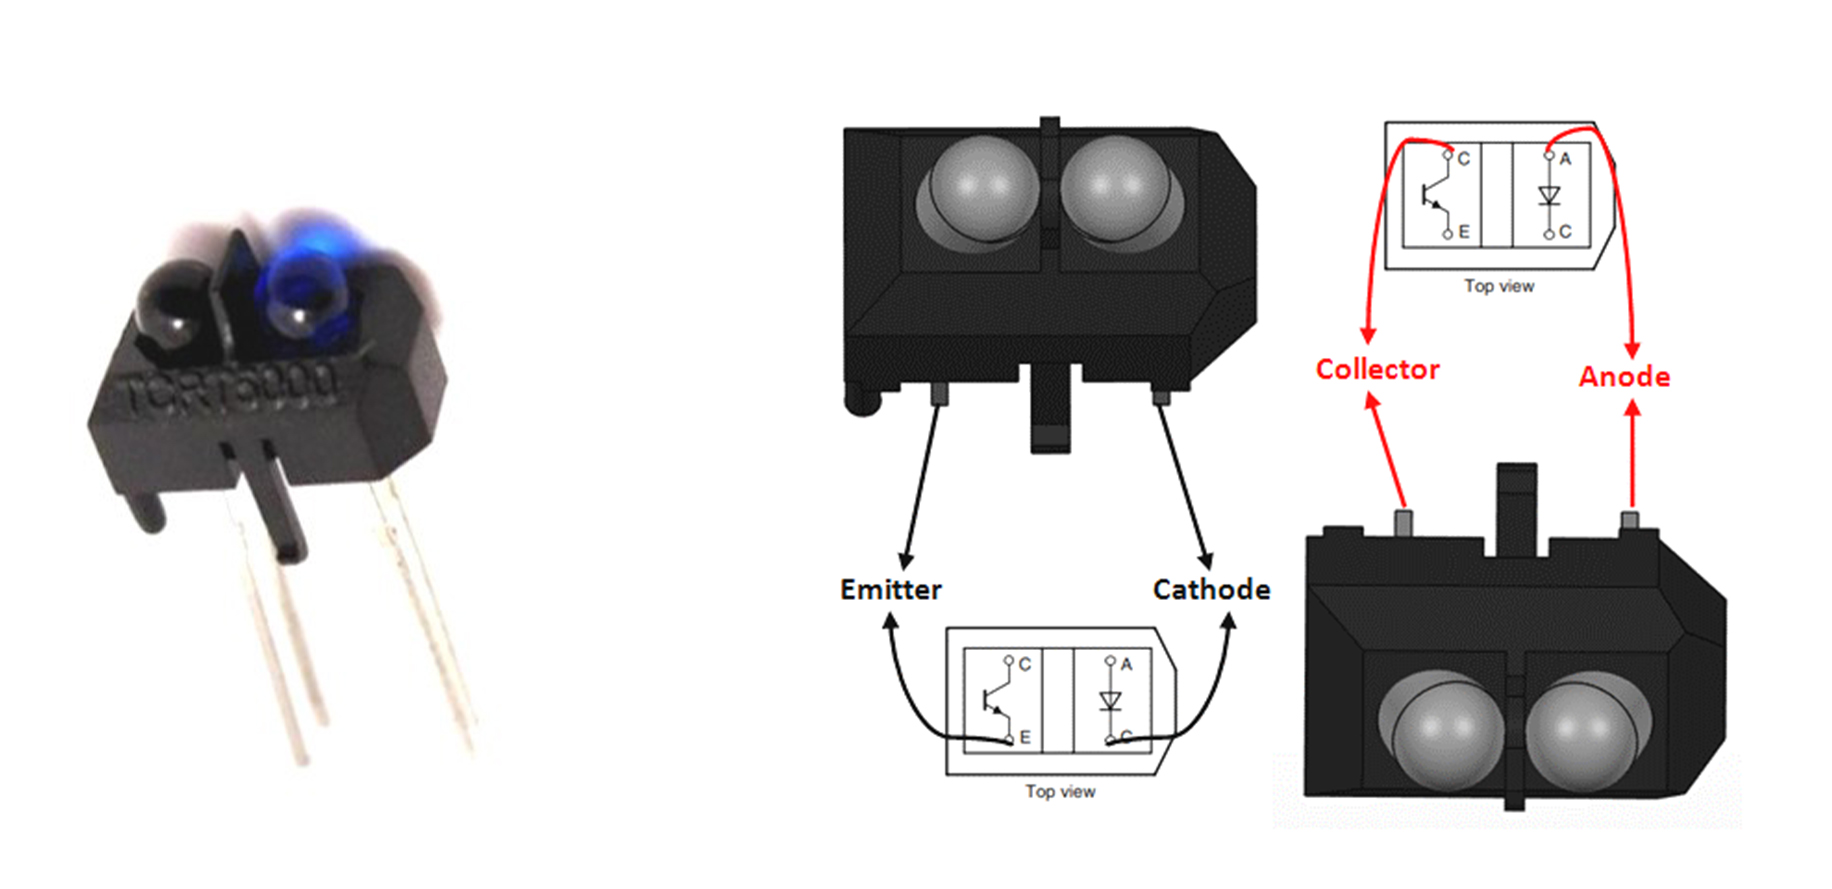
\includegraphics[scale=0.5]{figures/irsensor}
		\caption{TCRT5000 IR Sensor\cite{pinout}}
	\end{figure}
\end{center}

This sensor can be categorized as a  reflective sensors. It has both a Photo-diode and a Photo-transistor coupled in its package. Photo-diode is used as a emitter which emits IR beam which has around 950 nm wave length. This IR beam is reflected if it meets a reflective object. The reflected IR beam is then detected by Photo-transistor of TCRT5000 sensor. So this sensor is mostly used for detect presence of the object or any other reflective surface in front it. There are so many sensors which do the same purpose. They are,

\begin{enumerate}[1]
	\item \textbf{LED and LDR} : LED is used as a sender and LDR is used as a receiver. This combination is also good because it is more reluctant to sunlight noise. But the receiver output is not enough to detect perfectly for colors which has less difference from white. And also it must be calibrated frequently.
	
	\item \textbf{LASER DIODE and LDR} : Sender is a Laser diode and LDR is the receiver. In every way this combination perform very well. There are no issue from sunlight and also environment because laser beam has very high density. If the surrounding has same color which emits from the laser , there will be an error. And the laser diodes are expensive , so if we create sensor panels we have to spend considerable  amount of money.
	
	\item  \textbf{White color LED with high intensity and LDR} : When we use this combination there will be no issue from surrounding colors as other sensor combinations. Here also LDR is used as a receiver. High intensity of LED  prevents effects from sunlight. But for the optimum result we have to keep very low  distance between the sensor and surface.
	
	\item \textbf{IR LED and Photo-transistor (TCRT 5000)} : It was mention previously as topic. There is a issue also. It can recognize only white and black  with complete accuracy.
\end{enumerate} 

Considering all of these sensors and our task we can easily select IR sensors (TCRT 5000).  Its color sensing error does not valid for our task because it has only white lines on black background. TCRT 5000 sensor is covered and it blocks unwanted light which comes from the environment. And also the emitter and receiver are separate by each other to prevent unwanted reflections. So this one is more truthful and  efficient than other. And it  has a low cost. So it is better instead of (1) and (2) (mentioned above). Considering (3) it needs low distance. But our task has ramp area and we need required speed. So considering our task this combination (3) is not suitable for us.\\
In our project this sensor ( TCRT 5000 ) is used for detecting white line which is on the black background. White surface is known as reflective surface and black is not. So we can detect the presence of white lines. Our sensor panel configuration consists 8 IR sensors and each one has a special position. According to this placements robot brain can verify where the robot is. It has several specifications such as\cite{pinout},



\begin{table}[!h]
	\centering
	
	\begin{tabular}{l l}
			
		&\\
		IR sensor with transistor output&\\
		Operating Voltage&3V - 5V\\
		Diode forward Current& 60mA\\
		Output& Analog or digital  \\
		Transistor collector current& 100mA (maximum)\\
		Operating temperature&-25\degree C to +85\degree C\\
		Operating range& 0.2mm – 15mm\\
		Dimensions\cite{ir} ($ L*W*H $ in mm)& 10.2 x 5.8 x 7 \\
		&\\
	
	\end{tabular}
	
	\caption{ TCRT 5000 IR Sensor features and specs}
\end{table}	

When sensor is powered and began to sense, there will be an analog output which can also be vary according to environmental conditions (mainly day light ). Therefore it is not possible to guarantee 100\% accurate analog to digital conversion as we expect. So a \textit{comparator circuit} which consists of LM324 operational amplifiers is used in addition to the normal sensors to take clear digital output.














\section*{\underline{HC-SR04 Ultrasonic Sensor}}




This is a proximity sensor, also known as an ultrasonic transducer based on a transmitter and a receiver and mainly used to determine the distance to a target object. In our case, we use this sensor to detect distances to the colored box and to the walls in wall following part. So, we have to use three ultrasonic sensors to achieve this task. Two sensors are attached on the left and right sides of the robot to detect the distance to the wall. One sensor is attached in  front of  the robot to detect the distance to the box.\\
\begin{center}
	\begin{figure}[!h]
		\centering
		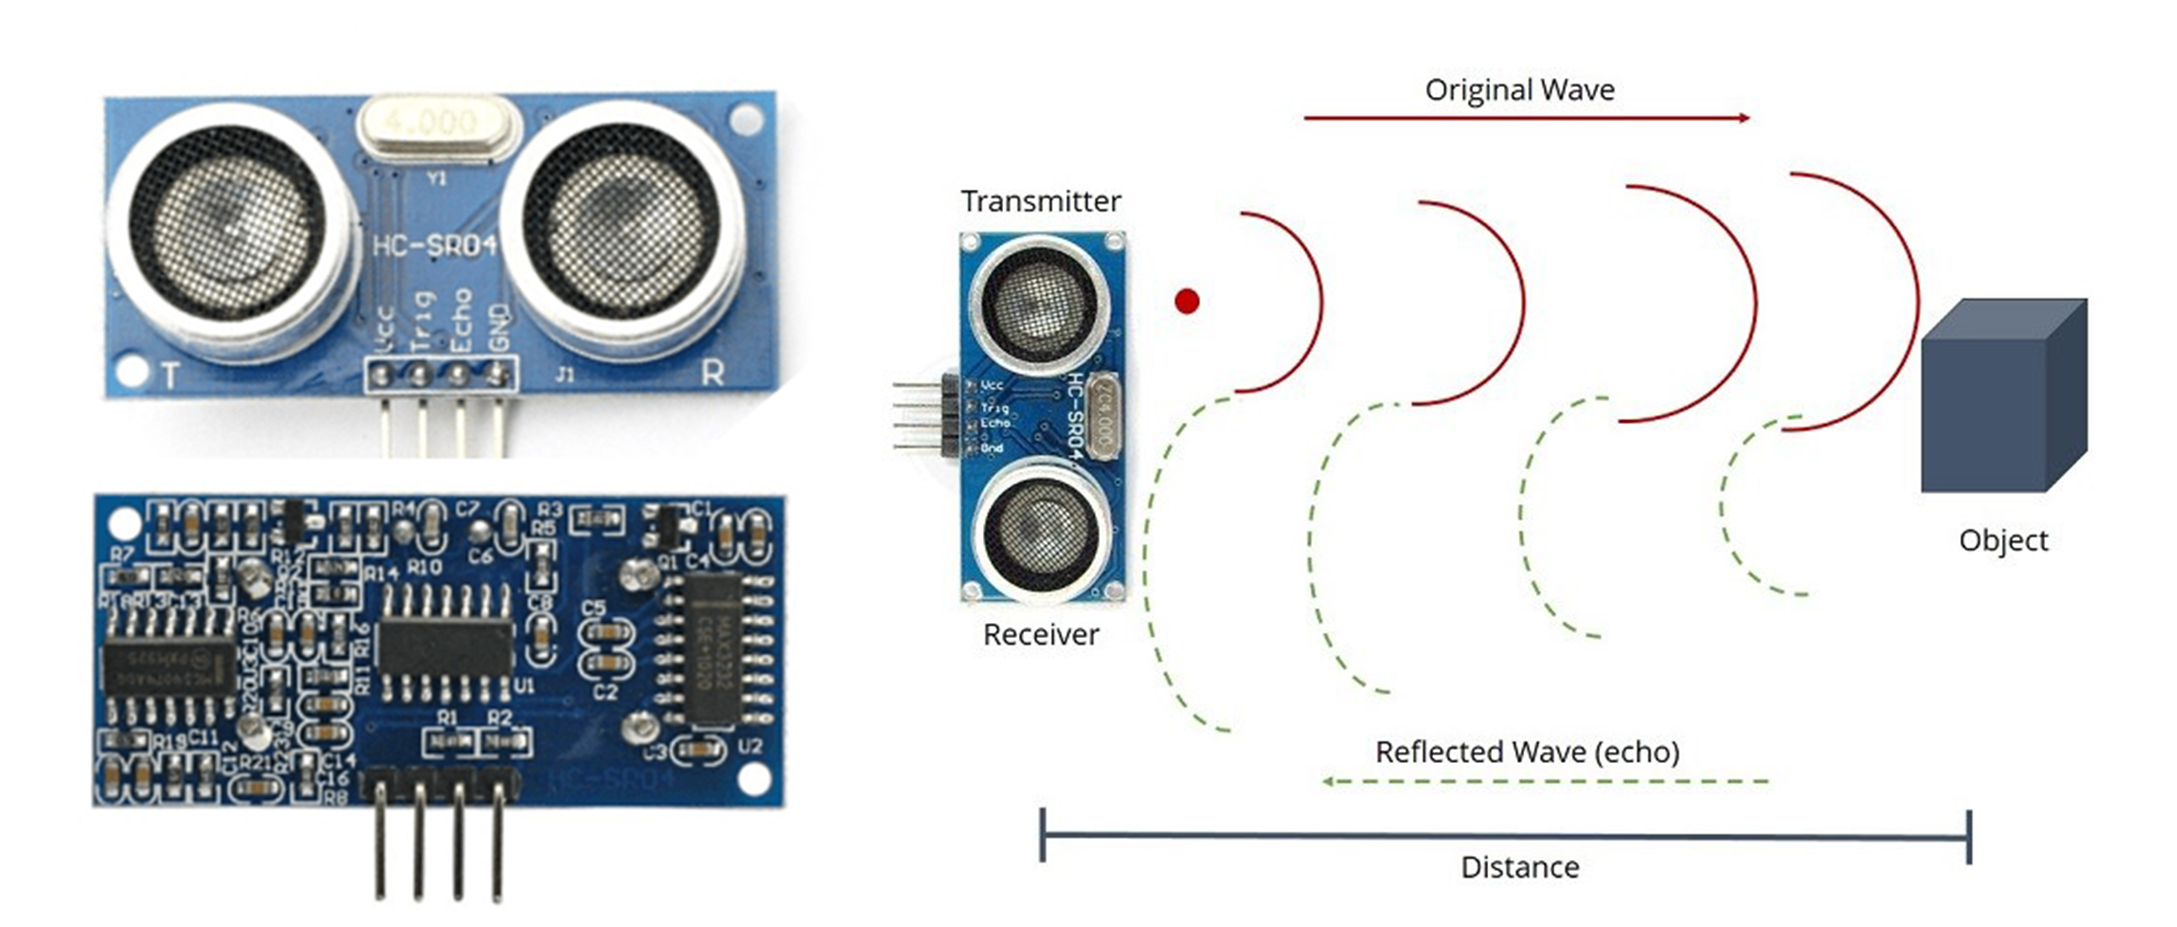
\includegraphics[scale=0.4]{figures/ul}
		\caption{HC-SR04 Ultrasonic Sensor and Its Object detecting Method}
	\end{figure}
\end{center}
It comes as a complete package with an ultrasonic transmitter and a receiver. The amount of time it takes to send and receive waves will determine how far the object is placed from the sensor. It mainly depends on the sound waves working on \textit{“non-contact” technology}. The required distance of the target object is measured without any damage, giving accurate and precise details. Here’s a list of some of the HC-SR04 ultrasonic sensor features and specs\cite{noauthor_complete_2018}.

\begin{table}[!h]
	\centering
	
	\begin{tabular}{l l}
		
		&\\
		Power Supply	&		+5V DC\\
		Quiescent Current 	&	 Less than 2mA\\
		Working Current	&	 15mA\\
		Effectual Angle	& Less than 15\degree \\
		Ranging Distance &		2cm – 400 cm/1'' – 13ft\\
		Resolution 		&		 0.3 cm\\
		Measuring Angle	&	 30 degree\\
		Trigger Input Pulse width&10uS\\
		Dimension		&		 45mm x20mm x15mm\\
		&\\
	
	\end{tabular}
	
	\caption{HC-SR04 ultrasonic sensor features and specs}
\end{table}	
	
	
Our need to use this sensor is to measure distances to obstacles. There are several different sensors that can perform this function as \textit{Infra-Red (IR) range sensor, Ultrasonic Sensor, Laser Range Sensor}. But, apart from the Ultrasonic sensor, there are some drawbacks when using other sensors. There are a lot of limitations in infrared sensors, like the inability to use them in sunlight due to interference\cite{noauthor_ultrasonic_2017}. Therefore, our measurements may change due to the light conditions in the environment.\\ Ultrasonic sensors work using sound waves, therefore detecting obstacles is not affected by many factors such as Light, Dust, Smoke, Mist, Vapor and Lint. So, the Ultrasonic sensor is more reliable than using the IR sensor. The Laser Range Sensor is better than these two sensors because it has higher accuracy and resolution  than the others. But we don't need that much precision or resolution for our task. Also, Laser Range Sensor is a high cost devise. So, the Ultrasonic Sensor is more effective than the others in achieving our purpose.


\section*{\underline{TCS34725 - Color Sensor}}




A Color Sensor is a device which detects or senses colors. A color sensor uses an external means of emitting light (like an array of white LEDs) and then analyses the reflected light from the object in order to determine its specific color.\\
There are many color sensors available. Some of them are \textit{TCS230, TCS3200} and \textit{TCS34725} etc. The TCS230, TCS3200 and TCS3210 senses color light, with the help of an 8 x 8 array of photo-diodes\cite{dejan_arduino_2016} and use a Current-to-Frequency Converter on the readings of it to  convert them into a square wave with a frequency directly proportional to the light intensity which is less accurate than the sensor TCS34725 that we use.\\ 
\begin{center}
	\begin{figure}[!h]
		\centering
		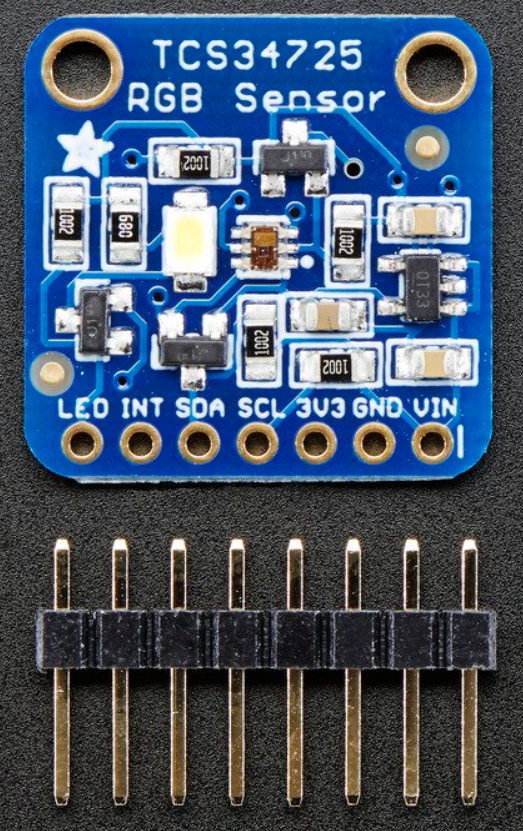
\includegraphics[scale=0.3]{figures/color}
		\caption{TCS34725 - Color Sensor}
	\end{figure}
\end{center}

An IR blocking filter, integrated on-chip and localized to the color sensing photodiodes, minimizes the IR spectral component of the incoming light and allows color measurements to be made accurately. The sensor additionally has an amazing 3,800,000:1 unique range with flexible incorporation time and increase so it is appropriate to use behind obscured glass. The high sensitivity, wide dynamic range, and IR blocking filter make the TCS34725 an ideal color sensor solution to use under varying lighting conditions and through attenuating materials. In addition, the IR blocking filter enables the TCS34725 to perform \textit{Ambient Light Sensing} (ALS). The TCS34725, itself, can enter a lower-power wait state between light sensing measurements to further reduce the average power consumption\cite{industries_rgb_nodate}.



\section*{\underline{MPU-6050 Gyroscope}}
\begin{center}
	\begin{figure}[!h]
		\centering
		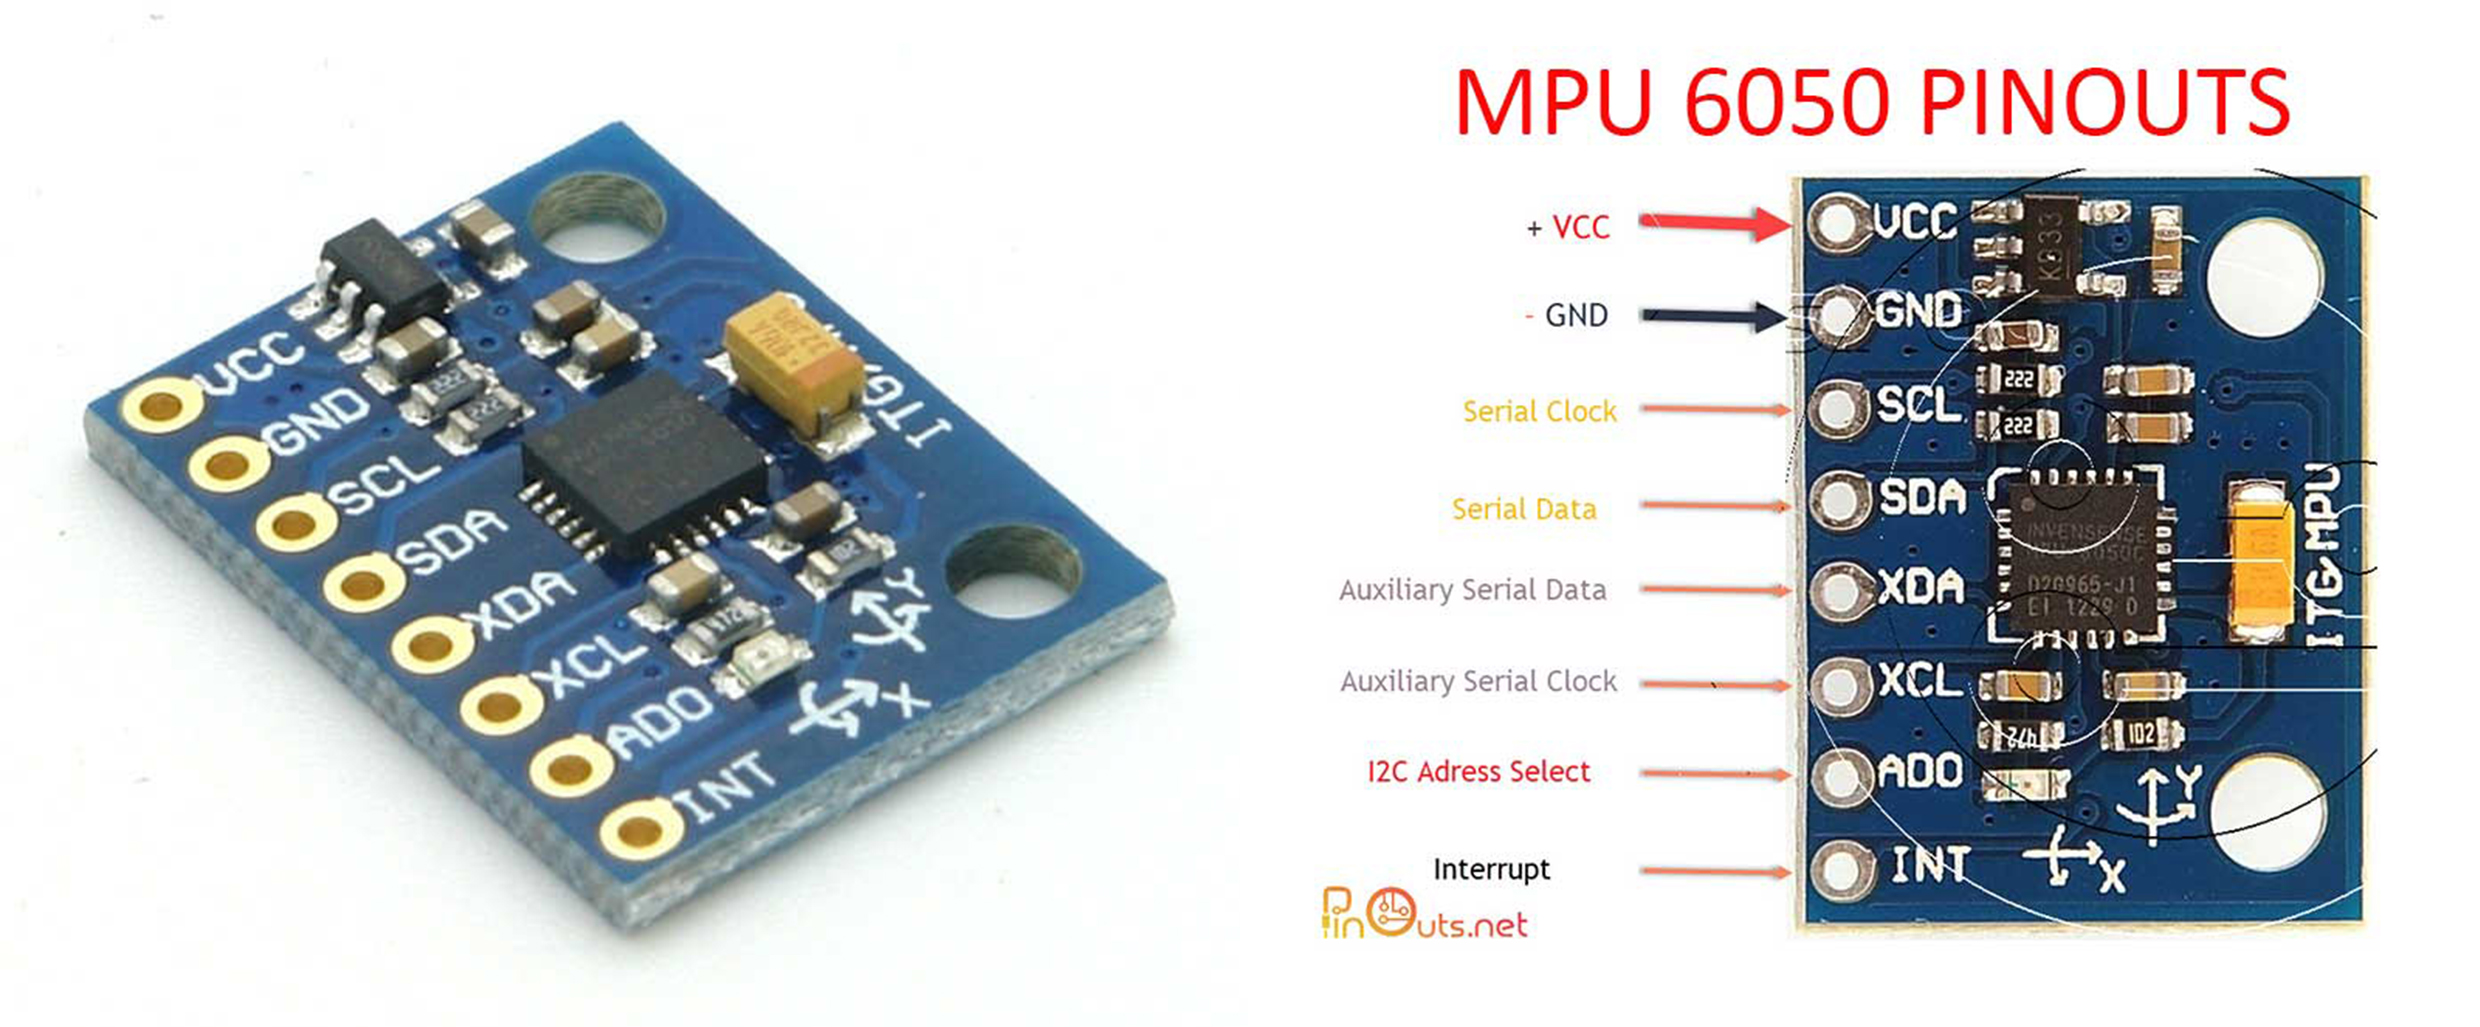
\includegraphics[scale=0.4]{figures/mpuu}
		\caption{MPU-6050 Gyroscope\cite{noauthor_mpu6050_nodate} with its Pinout\cite{admin_mpu6050_2019}}
	\end{figure}
\end{center}
This sensor is used to identify the angle of the robot and giving a feedback so that the motor speed of the robot could be changed likewise. This is very useful in the ramp activity, so that the speed of the robot can be controlled. The MPU-6050 consists of a 3-axis gyroscope and a 3-axis accelerometer on the same silicon die, together with an onboard Digital Motion Processor capable of processing complex 6-axis motion fusion algorithms. The device can access external magnetometers or other sensors through an auxiliary master I2C bus. If 3-axis Magnetometer is connected to auxiliary I2C bus, then MPU6050 can provide complete 9-axis Motion Fusion output. This has a built-in voltage regulator\cite{noauthor_gyroscope_2019}.\\
There are some other types of gyroscope sensors too that can be used for this purpose such as, 
\begin{enumerate}[1]
	\item ADXL335
	\item ADXL345
	\item MMA7361
	\item LIS3DH Triple-axis accelerometer module
\end{enumerate}

	
All above modules are 3-axis gyroscopes and 3-axis accelerometers. ADXL 335, ADXL345 are low power consumption sensor modules. The modules generate separate analog voltage for each axis. MMA7361 has a sleep mode and a select pin which can be helpful to save power. Above three modules have low power consumption and easy to use and program but do not have  onboard digital motion processors (DMP) unlike MPU-6050. So, as we need an onboard DMP for control of the robot above three modules are not much of a use. The LIS3DH module is an intelligent, low-power, capacitive, micro-machined accelerometer with 12-bit resolution. But this module also doesn’t have a digital motion processor like MPU-6050. So MPU-6050 is the most suitable gyroscope sensor for the project\cite{noauthor_mpu-6050_nodate}.

\bibliographystyle{plain}
\bibliography{ref}




\end{document}